%!TEX root = project.tex

\chapter*{About this project}
\paragraph{Abstract}
Data visualisation has become popular, in part due to everyone's experience with the global pandemic Covid-19. Information is delivered in easy to understand visual representations. As this is an emerging area, the team decided to investigate different methods of data visualisation, see which performed the best for different scenarios and to develop a data visualisation application. The main focus of the application is on Covid-19, data is being generated at least daily worldwide for Covid-19. The application includes examples of other pandemics such as SARs, MERs and historic epidemics of smallpox and polio.

\paragraph{Authors}
This project was developed as part of a fifteen credit module by Grace Keane, Jina Kim and Shirin Nagle, fourth year students of Galway Mayo Institute of Technology.

\paragraph{Acknowledgements} The authors would like to acknowledge the time and advice given by the project supervisor Dr. John French.

\chapter{Introduction}
This chapter will serve as a prelude to the project. The context, objectives and metrics for success and failure will be defined, followed by a thorough summary of the project domain and an introduction into each chapter of the dissertation and its relevance.

\section{Context}
During the decision making process the team decided that the project must be relevant as well as interesting. The project must encourage the use of existing skills as well as allow for the natural development of new and relevant techniques and processes while also being worthy of scope.

\vspace{5mm} %5mm vertical space

Data visualisation and analysis techniques have been the front and center in the efforts to communicate the statistics as well as the science around the COVID-19 virus. Interactive dashboards with several charts and graphs surfaced in different formats to offer concise ways to make sense of complex and overwhelming pandemic data sets. These techniques have become essential in informing the general public as well as healthcare providers, scientists and governments of the overall COVID-19 growth.

\vspace{5mm} %5mm vertical space

As a result, the team felt it would be beneficial as well as informative to create a web application that would take large COVID-19 data sets as well as other pandemic data and create a series of data visualisations from it. As well as compare past and present viruses to distinguish similarities along with differences. This would provide a clear view of COVID-19 and how similar viruses have spread.

\vspace{5mm} %5mm vertical space

Once the project area had been decided on, each team member focused on a pandemic or epidemic, investigated where to source relevant information for the pandemic or epidemic, and investigated different technologies for displaying data in a visual manner.

\section{Project Objectives}
As previously mentioned, the end goal of the project is to create a web application that would process different virus data and create various data visualisations to ensure a simple way for users to view large complex pandemic data. To ensure the end goal was reached, the team outlined objectives to be followed post development.

\begin{itemize}
  \item Investigate the field of interest and scope for the project.
  \item Evaluate and research the appropriate frameworks and tools available for development.
  \item Incorporate state of the art technologies, frameworks, databases and tools that will allow users to view, add, update, delete, post and retrieve data.
  \item The web application will, at a minimum allow users to sign-up, login, view data visualizations as well as incorporate user interaction features, create unique user visuals and post user data to databases.
\end{itemize}

\section{Metrics for Success and Failure}
The outlining criteria for success and failure were important in ensuring the project remained on track throughout development and therefore allow the project to achieve the outlined goals in a timely and standard-driven manner. The defined metrics are of similar nature to that of the underlying objectives defined in \emph{Section .....} but explained at a higher level.

\vspace{5mm} %5mm vertical space

\subsection{Applied Project Dissertation}
A selection of metrics were outlined specifically for the dissertation, they are as follows.

\begin{itemize}

    \item \emph{The final dissertation should be easily understood, allowing readers without knowledge or familiarity of the subject area to form a suitable understanding of the concept and areas discussed.} In order to accurately measure this metric, input was received from family and fellow students, who would kindly read newly integrated sections and provide useful feedback.

    \item \emph{The  dissertation should be in order of 10,000 - 15,000 words, excluding appendices as well as approximately 105 pages (excluding diagrams, abstract, TOCs, references, appendices etc.)}

\end{itemize}

\subsection{Applied Project}
A selection of metrics were outlined specifically for the development of the applied project, they were as follows.

\begin{itemize}

    \item \emph{The applied project must be easy to use, navigate and attempt to deal with a task of problem deemed to be of sufficient technical challenge and depth.} To ensure this was adhered to, at frequent stages of development feedback from fellow students and Dr. John French was considered and documented relating to the application.

    \item \emph{Collaboration between team members and supervisors should be consistent to ensure a smooth work flow throughout the project planning and development.)} In order for this metric to be adhered to, the team maintained communication with themselves and Dr John French throughout the development and planning of the applied project.

\end{itemize}

\section{Dissertation Summary}
This section will contain a brief overview of the dissertation structure and will provide a short description of each chapters objectives.

\subsection{Methodology}
In this chapter, the processes undertaken during the life cycle of the project regarding planning, testing and development will be outlined. Investigating development methods and methods employed during the research phase, their results and the effect they had on the direction of the project will be brought to the attention of the reader. Additional, the decisions, thought process and influential factors leading up to those processes and design implementations will also be described.

\subsection{Technology Review}
A technological review will encapsulate the technical aspect of the project. This includes the different technologies incorporated, their implementation, their roll, and why they were chosen. The benefits of the chosen technologies will be critically analysed and compared with similar alternatives.

\subsection{System Design}
A detailed explanation of the overall system architecture will be provided. Diagrams will be included to help illustrate and explain the inner workings of the application at a high level.

\subsection{System Evaluation}
An evaluation of the final applied project against the initial project objectives. The final result of the project will be critically analysed including an analysis of areas of software quality, improvements or changes to the overall project.

\subsection{Conclusion}
To conclude, a brief summary of the context and objectives to remind the reader about the overall rationale and goals of the project. Key insights will be identified and reflected on. A final analysis will describe the teams overall experience and what the team learned while working on a project similar to one encountered in the software industry.


\chapter{Methodology}
The first project meeting took place in the final week of September 2020. This meeting consisted of analysing the applied project requirements that had been defined and outlined. The team agreed to choose a topic that would be informative yet beneficial to the end user. It was concluded that the final idea and architecture of the solution should be finalised as soon as possible to allow for necessary research and planned development.

\vspace{5mm} %5mm vertical space

This chapter will explore the pre-development process, the approach the team took with development and testing, how the team dealt with various problems faced, and the influence of regular supervisor meetings along with a conclusion based what impact pre-development research had on the overall project direction.

\section{Technological Brainstorming and Initial Supervisor Meeting}
Before development began and after the initial project topic was chosen each team member researched various technologies and concepts that could be potentially incorporated into the project. Soon after a brainstorming meeting was conducted to critically analyse each technology researched and the team decided whether each would be of good fit.

\vspace{5mm} %5mm vertical space

The team met prior to the initial supervisor meeting to produce effective ideas and questions to be asked relating to the overall architecture of the solution and the ultimate goals and objectives, these included:

\begin{itemize}

    \item \textbf{What research areas should be prioritised before development is conducted?}

    \item \textbf{What technologies would be of best fit for the project?}

    \item \textbf{What benefits would certain methodologies posses compared to others?}

\end{itemize}

During the initial supervisor meeting the project idea, potential research, development technologies, development methodology and collaboration approaches were discussed. The team were advised to spend the next few weeks to consider and finalise the overall nature of how the applied project will be designed and implemented.

\vspace{5mm} %5mm vertical space

After the supervisor meeting the team decided to take this advise on board. Each member focused on researching the What? Why? How? of the project technology, idea and the overall end user experience as well as the relevance of the project. Once research was carried out the team had a meeting to discuss and critically analyse the findings. Some questions asked were as follows:

\begin{itemize}

    \item \textbf{What development methodology and collaboration technique would be best to adapt?}

    \item \textbf{Would the chosen project idea be of relevance to the end user?}

     \item \textbf{Would the chosen technologies be of a professional standard?}

    \item \textbf{How would the chosen technologies fit together as a whole?}

    \item \textbf{Is the scope an appropriate size for a three person project?}

\end{itemize}

\section{Methodology Consideration}
There where numerous possible methodologies to consider. After discussions with team members, the team agreed to critically analyse and compare \textbf{Waterfall} and \textbf{Agile} to determine which methodology would be of best suit to the applied project.


\vspace{70mm} %5mm vertical space


\section{Determining Development Methodology}
Following the decision of Agile and Waterfall as an approach to software development, the team began to research the advantages and disadvantages of both, along with deciding which methodology would be best to take when considering the scope, project goals and time frame. A critical analysis and overview of both methodologies were made and a conclusion based on the practical analysis of each in relation to the project was undertaken.

\section{Waterfall}
The Waterfall model is composed of a series of steps, illustrated in \emph{Figure....}. These steps are used to break down a project into linear sequential phases to ease the development process.  \cite{petersen2009waterfall}. Waterfall allows progress to be easily measured, the complete scope of the project is known in advance, which can be preferred based on the type of project and software team. The Waterfall model tends to be among the less flexible approaches, the output of each stage completed is the input for the next and the overall progress follows a fixed downwards path like a waterfall.

\begin{center}
      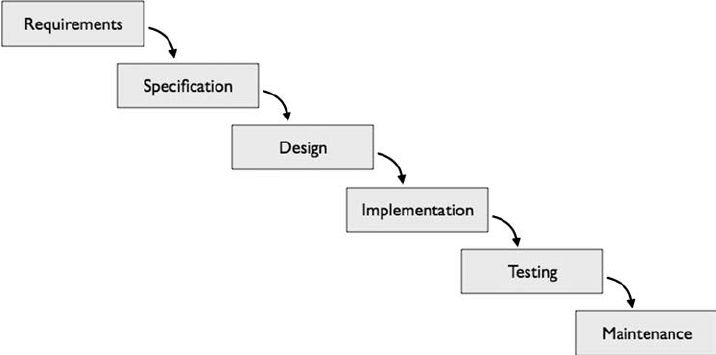
\includegraphics[scale=0.46]{img/Waterfall.png}
\end{center}
\label{fig:x cubed graph}

The waterfall model is still a widely used method for working on software projects today. It is arguably the most well known development model, which is likely attributed to how long the model has been around, not to mention the overall simplicity of the model. Each phase is of a waterfall project is completed sequentially and testing is done after tasks are completed. \cite{balaji2012waterfall}.


\section{Agile}
Agile methodologies are a group of software development methods that are based on interactive and incremental development \cite{kumar2012impact}. The term agile stands for 'moving quickly'. It is characterised by an approach that allows rapid and continuous delivery of small and useful software. It takes the view  that production teams should start with simple and predictable approximations to the final requirement and then continue to increment the detail of these requirements throughout the life of the project. Agile methodology has an adaptive team which is able to respond to changing requirements as well as the ability to solve problems even late in the development cycle. \cite{balaji2012waterfall}.
\begin{center}
      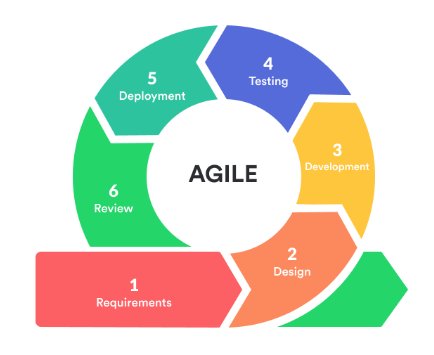
\includegraphics[scale=0.8]{img/Agile.png}
\end{center}
The popularity of Agile development methodologies amongst the software industry has increased drastically, with almost 85.4\% of international surveyed software developers using Agile methodologies in their work. \cite{agileStats} Research has also shown that Agile projects are 28\% more successful than traditional projects. The most important principle of the Agile methodology is customer satisfaction by giving rapid and continuous delivery of small and useful software.

\section{Comparison between Agile and Waterfall}
Following team meetings, research and analysis, both Agile and Waterfall were critically analysed under the following headings:

\begin{itemize}

    \item \textbf{Requirement delivery}

    \item \textbf{Flexibility}

    \item \textbf{Compatibility}

     \item \textbf{Methodology past experience}

\end{itemize}

By taking the above headings into an account comparisons were drawn of both methodologies.

\begin{table}[ht]
  \centering
  \begin{tabular}{x{5cm}p{5cm}}
    \toprule \\
    Agile & Waterfall \\
    \midrule \\
    + Ability to respond to the changing requirements of the project. & + Requirements are clear before development starts. \\
    + Errors can be detected and solved quickly. Which is a big advantage. & + Each development phase is completed in a set time frame. Then it moves to another phase. \\
    + There is constant communication and inputs from the team and supervisor & + It is a linear model so therefore easy to implement. \\
    - Project can easily fall off track. & - Requirements, Specification and Design can take up a lot of time. \\
    - The end point of the project is not clearly defined. & - Low flexibility meaning it may be difficult of even impossible to make major changes while in the implementation phase \\
    \bottomrule
  \end{tabular}
  \caption{A table.}
  \label{table:mytable}
\end{table}


Following various comparisons between the Agile and Waterfall, it became clear to the team that an Agile approach would best suit the development of the outlined applied project. This approach would aid the development process in numerous ways, these include:

\vspace{70mm} %5mm vertical space

1. \textbf{Errors can be detected and solved quickly} - The team thought it would be beneficial to be able to detect and solve problems quickly, especially when the team did not have much experience with using GitHub collaboratively together as a team.

2. \textbf{The ability to develop small but functional software via releases} - Based on feedback from our supervisor the priorities of the project would be subject to change. Small incremental changes means there would be flexibility and versatility throughout the development stage.

3. \textbf{GitHub project boards and Scrum Methodologies} - The idea of incremental releases in parallel with scrum sprints based on workflow defined in GitHub project boards was something the team thought would be of major benefit to the overall workflow.

4. \textbf{Frequent supervisor and team meetings} - Information sharing in teams is an important aspect of successful software development. The team felt it would be crucial to hold regular team meetings to discuss what each member is working on as well as attend all weekly supervisor meetings.

\subsection{Agile Methodology}
Deciding what exact agile methodologies was the next big step the team had to decide on. After research the team came to a conclusion that Scrum and GitHub project tasks would be of most benefit.


\subsection{GitHub Tasks}
Since the beginning of development for the applied project the team set up and adhered to GitHub tasks by assigning relevant work to do each week. GitHub tasks also knows as GitHub Kanban is a project management tool designed for developers to coordinate, track and update their work in one place, so projects stay transparent and on schedule.

\vspace{5mm} %5mm vertical space


It provides tools to allow developers to prioritize and visualize the main elements of the project in progress and also created a clear picture of what project tasks need to be started, completed and which tasks are currently in progress. 

https://github.com/features/project-management/

\vspace{50mm} %5mm vertical space

The ability to track project progression on the same platform where the project is being collaborated on is a huge benefit as well as more efficient than using an external project management tracker. 

\begin{center}
      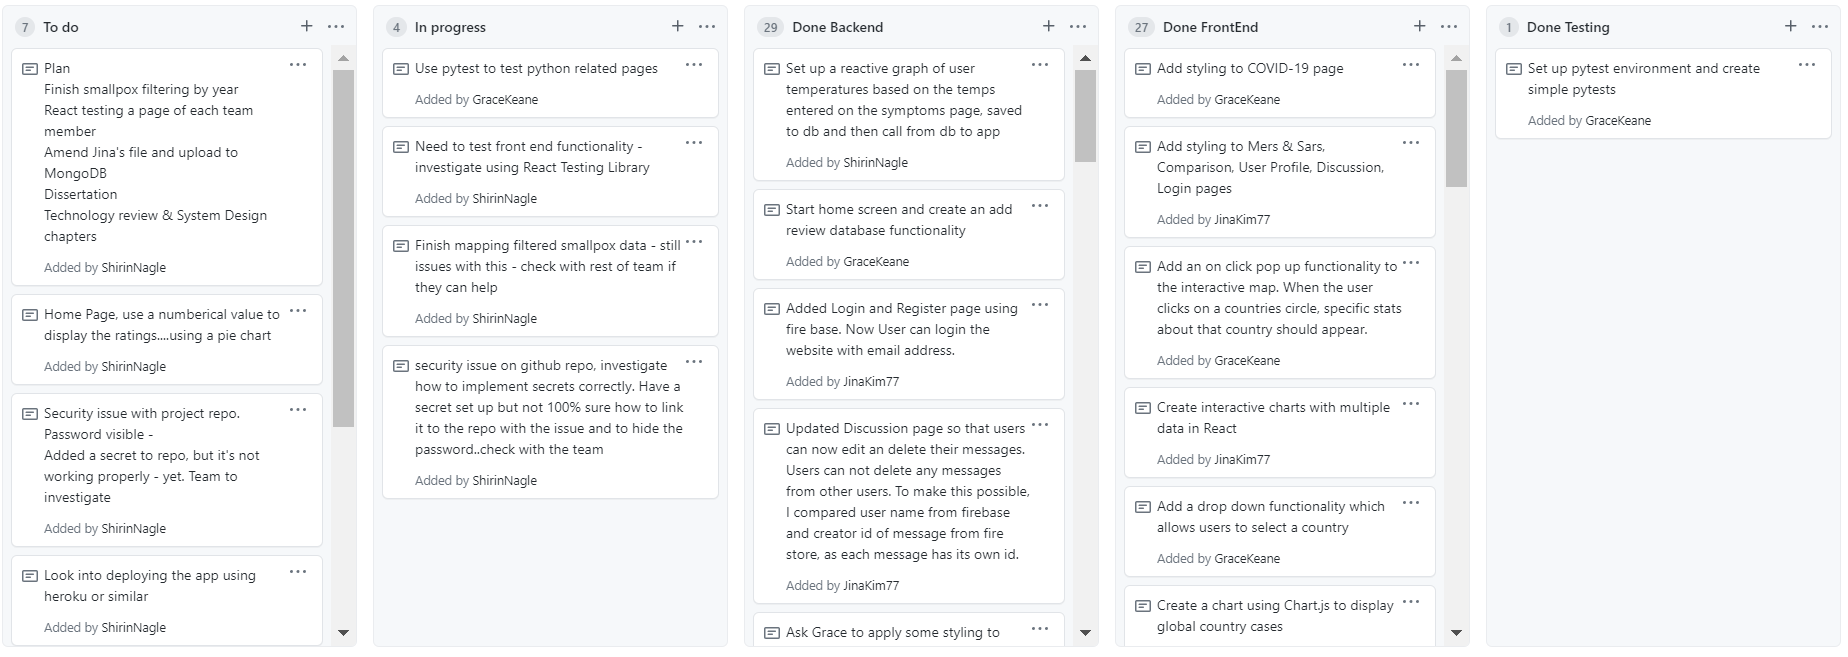
\includegraphics[scale=0.50]{img/GitHubToDo.PNG}
\end{center}
\label{fig:x Github Tasks}
<<<<<<< HEAD

The figure above shows the GitHub task sheet used during development of the applied project. It consists of five main columns:

\begin{itemize}
\item \textbf{To Do}
\item \textbf{In Progress}
\item \textbf{Done Backend}
\item \textbf{Done Frontend}
\item \textbf{Done Testing}
\end{itemize}
=======

The figure above shows the GitHub task sheet used during development of the applied project. It consists of five main columns:

\begin{itemize}
\item \textbf{To Do}
\item \textbf{In Progress}
\item \textbf{Done Backend}
\item \textbf{Done Frontend}
\item \textbf{Done Testing}
\end{itemize}

\subsection{Scrum}
As well as using GitHub Tasks to manage project management, the Scrum methodology was incorporated and employed. The Scrum methodology contains the same concepts as agile \ref{mahalakshmi2013traditional}. It is designed for teams to break down work into goals that can be completed in a specific time frame called sprints. Sprints are generally one week in length. At the end of each week, a supervisor meeting would be held where the team would discuss their progress with the supervisor.

\vspace{5mm} %5mm vertical space
>>>>>>> 56dd2e8b5180e8056eea060c041318782e4ed604

\subsection{Scrum}
As well as using GitHub Tasks to manage project management, the Scrum methodology was incorporated and employed. The Scrum methodology contains the same concepts as agile \ref{mahalakshmi2013traditional}. It is designed for teams to break down work into goals that can be completed in a specific time frame called sprints. Sprints are generally one week in length. At the end of each week, a supervisor meeting would be held where the team would discuss their progress with the supervisor.

\vspace{5mm} %5mm vertical space

At the end of each supervisor meeting, the goals for the next Scrum Sprint were defined and discussed in detain. Any new goal was also assigned and recorded in the teams GitHub Tasks board. These tasks were undertaken in a high to low priority order.

At the end of each supervisor meeting, the goals for the next Scrum Sprint were defined and discussed in detain. Any new goal was also assigned and recorded in the teams GitHub Tasks board. These tasks were undertaken in a high to low priority order.

\vspace{70mm} %5mm vertical space



About one to two pages.
Describe the way you went about your project:
\begin{itemize}
\item Agile / incremental and iterative approach to development. Planning, meetings.
\item What about validation and testing? Junit or some other framework.
\item If team based, did you use GitHub during the development process.
\item Selection criteria for algorithms, languages, platforms and technologies.
\end{itemize}
Check out the nice graphs in Figure \ref{tikz:graphs}, and the nice diagram in Figure \ref{tikz:mydiagram}.



\chapter{Technology Review}
This chapter will outline the technology used and the reasoning for choosing a particular technology. Below is a list of technologies used, descriptions of the technologies at a conceptual level are included for each technology.
\begin{itemize}
\item Git
\item GitHub
\item React
\item Flask
\item MongoDB
\item FireBase
\item FireStore
\item D3
\item JavaScript
\item Python
\item Visual Studio Code


\end{itemize}

\section{Version Control}
Version control is an essential element of any collaborative undertaking. An organisation in GitHub was set up to manage the version control for the project. At the early stages the team were investigating different aspects of data visualisation, when this investigation concluded we created a new repository where all the future work of the project would be tracked.
\subsection{Git}
Git is a free and open source distributed version control system designed to handle everything from small to very large projects with speed and efficiency. It is a free and open source software distributed under the terms of the GNU General Public License version 2.
Git allows and encourages the user to have multiple local branches that can be entirely independent of each other. The creation, merging, and deletion of those lines of development takes seconds. [SN 1]
Git is installed and maintained on the users local system and provides a record of ongoing programming versions. It allows developers to rollback to an older version of the code if required.
There are other popular version control systems for example Apache SVN or CVS, the team chose Git as it was a technology that we were familiar with but did not have a lot of experience with. We felt that there would be many large learning curves ahead of us and if we could mitigate the size of the learning curve by choosing a familiar technology it would help us focus on other areas that required more learning. Having said that there was a significant learning curve using Git with a team. Git gave us experience of using branches, merging branches and manually resolving conflicts.
\begin{figure}
    \centering
    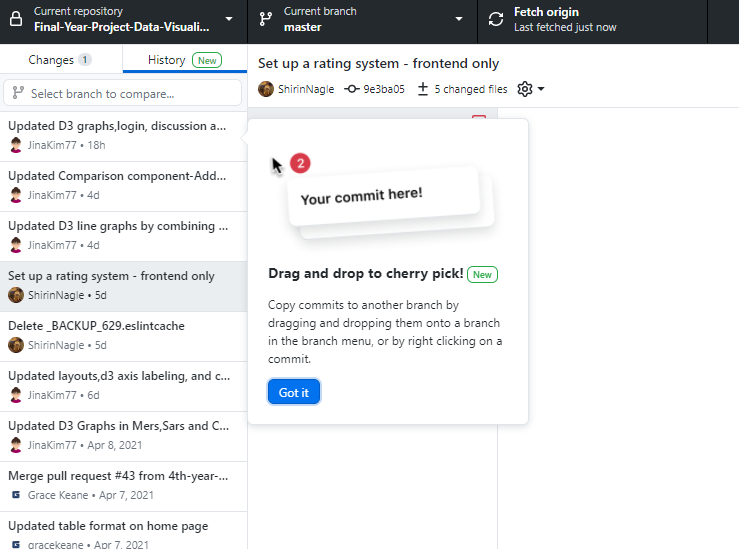
\includegraphics[scale=0.7]{img/git.PNG}
    \caption{Git on local machine}
    \label{fig:my_label}
\end{figure}



\subsection{GitHub}
GitHub is a web based code hosting platform for version control and collaboration. It lets users work together on projects from anywhere.[SN 2]
GitHub provides students of GMIT with free accounts, for this project a free account was sufficient as there is a facility to make the project public or private. Using GitHub allowed the team to work entirely remotely.
\begin{figure}
    \centering
    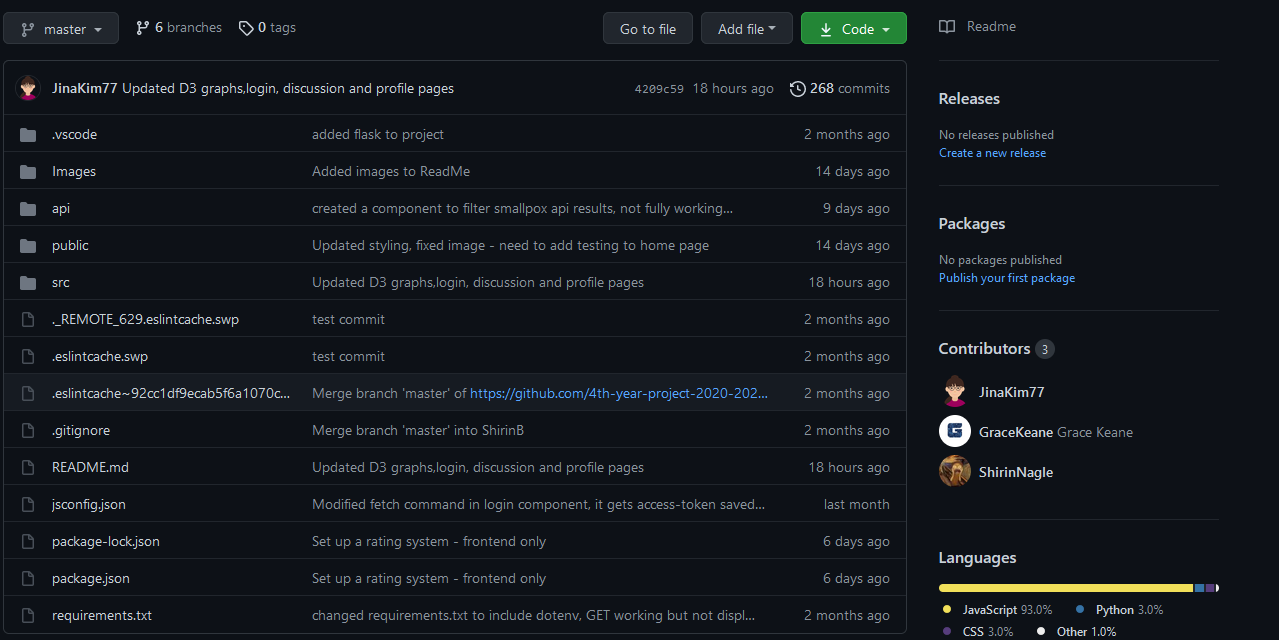
\includegraphics[scale=0.5]{img/github.PNG}
    \caption{Github Organistaion}
    \label{fig:my_label1}
\end{figure}





\subsection{Flask}
Flask is a micro web framework written in Python. It is classified as a microframework because it does not require particular tools or libraries. The “micro” in microframework means Flask aims to keep the core simple but extensible. It has no database abstraction layer, form validation, or any other components where pre-existing third-party libraries provide common functions. However, Flask supports extensions that can add application features as if they were implemented in Flask itself. Extensions exist for object-relational mappers, form validation, upload handling, various open authentication technologies and several common framework related tools.[SN 3]
The architecture of our project required a back end,front end and a database. We had some experience with MEAN and MERN stacks from previous college projects. More recently we had some exposure to Flask as a backend in Emerging Technology project. We had decided to use React for our frontend, which we had used for a previous MERN(Mongo, Express, React, NodeJs) project. We had also used Angular previously for a MEAN(Mongo, Express, Angular, NodeJs) project but decided to use React.There will be further discussion in the React section about why React was chosen. Part of the teams learning objectives was to use new technologies, to the team, and learn as much as possible about them. For this reason we chose Flask as our backend, as it offered flexible options re database and front end choices. From implementing Flask and reading documentation, the idea of virtual environments was introduced. Virtual environments are independent groups of Python libraries, one for each project. Packages installed for one project will not affect other projects or the operating system’s packages.[SN 4]
Most importantly using Flask allowed us to write our own API calls to our MongoDB Atlas database.

\begin{figure}
    \centering
    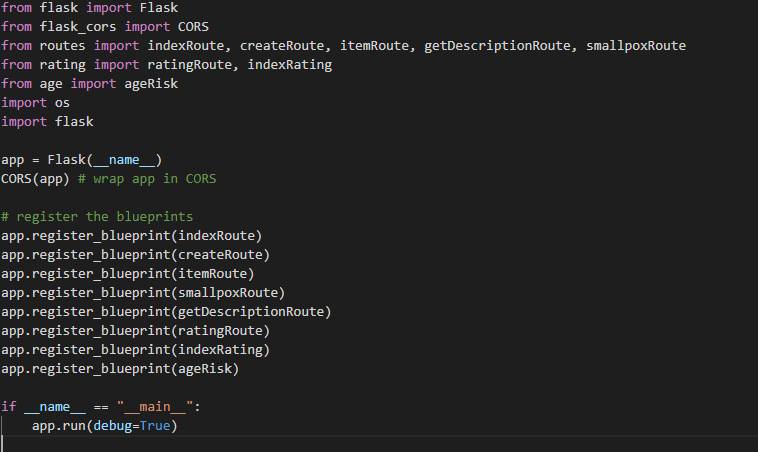
\includegraphics[scale=0.5]{img/flask.PNG}
    \caption{Flask}
    \label{fig:my_label2}
\end{figure}















\subsection{React}
React is a JavaScript library, used for building reusable components.React allows users to design simple views for each state in their application, and React will efficiently update and render just the right components when the data changes.
Declarative views make the code more predictable and easier to debug. Build encapsulated components that manage their own state, then compose them to make complex UIs.
React does not make assumptions about the users technology stack, allowing the development of new features in React without rewriting existing code. [SN 5]
React recommends using JSX, an syntax extension of Javascript. We have used JSX in our project.
See example code from the project.
\begin{figure}
    \centering
    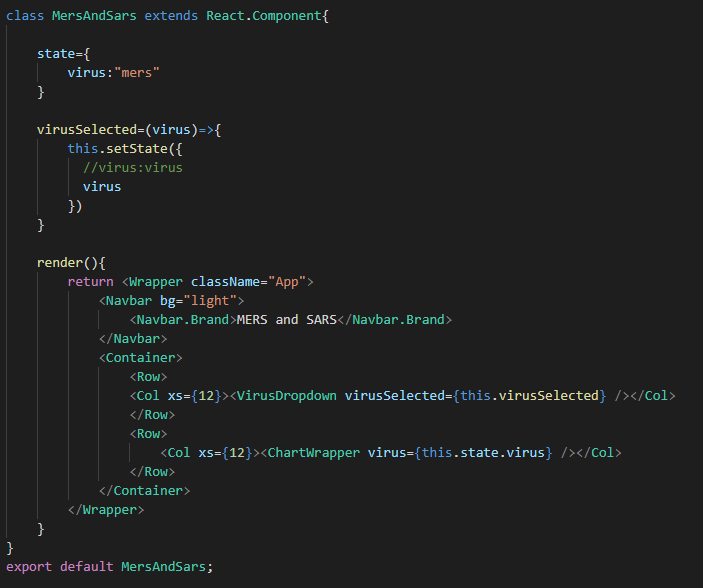
\includegraphics[scale=0.6]{img/jsx.PNG}
    \caption{Example of JSX}
    \label{fig:my_label4}
\end{figure}



When researching what front end software to use we considered Angular and React. From our research we compared the two technologies. Included below is a table outlining the advantages and disadvantages of both.
\begin{table}[ht]
\centering
\begin{tabular}{ |p{3cm}||p{3cm}|p{3cm}|p{3cm}| }
 \hline
 \multicolumn{4}{|c|}{FrontEnd Technology Comparison Angular v's React} \\

 \hline
 Heading& React& Angular&Best Option\\
 \hline
 Structure   & JS Library    &Full framework &  React\\
 Application & Suits SPA    & Suits large App   &React\\
 Updates &Often & Twice a year&  React\\
 Components and Size    &Uses virtual DOM & Uses Real DOM&  React\\
 Industry Demand&   897  & 366& React\\
 Professional Popularity& 68.9\% &54\%   &React\\
 Dubug& Easy& Not so Easy& React\\

 \hline
\end{tabular}
\end{table}

\hfill \break


Information about Job popularity taken from a google search on the 15th of April 2021
Information about professional popularity taken from StackOverflow survey(2020) of most loved Web framework.[SN 6]


There is no definitive way to decide in advance, which technology would be the best to use, but comparing relevant aspects between technologies can help narrow the choices and help with making the final decision. Having considered all of the information from the table above and taking into account our previous experiences with both Angular and React we chose React as our front end development technology.
Choice of FrontEnd Technology - can be looked at from 2 perspectives 1. A learning outcome.
2. A good fit for the task we were trying to achieve within the project.

Having completed the project, we feel it had been a good choice from both of those perspectives.

\subsection{MongoDB Atlas}
MongoDB Atlas is a database as a service, a cloud based service.
When designing the application we were unsure what format our data would take, if the data was purely relational it would only need a SQL type database, if the data was non relational it would need a noSQL database.
NoSQL databases (aka "not only SQL") are non tabular, and store data differently than relational tables. NoSQL databases come in a variety of types based on their data model. The main types are document, key-value, wide-column, and graph. They provide flexible schemas and scale easily with large amounts of data and high user loads.  NoSQL databases can store relationship data—they just store it differently than relational databases do. When compared with SQL databases, many find modeling relationship data in NoSQL databases to be easier than in SQL databases, because related data doesn’t have to be split between tables. he simplest type to describe is the document database, in which it would be natural to combine both the basic information and the customer information in one JSON document. In this case, each of the SQL column attributes would be fields and the details of a customer’s record would be the data values associated with each field.

For example: Last\_name: "Jones", First\_name: "Mary", Middle\_initial: "S", etc .


[SN 7] \\
For our data storage we decided to use a noSQL Database as this stored data in the way we required. We could have created a cloud based sql database using something like Postgres, but the amount of data we were handling did not require separation.
In the end most of our data was relational data but we felt that MongoDB Atlas was still a good fit as it allowed us to add other noSQL type data if the need arose. Each document has a different number of fields, size, content, and is stored in a JSON like format called BSON. The documents in MongoDB do not need to have a schema defined beforehand. The fields can be created on the fly. The data model available within the MongoDB allows developers to represent the hierarchical relationships, store arrays, and other more complex structures easily.
The mongo shell is an interactive JavaScript interface to MongoDB. You can use the mongo shell to query and update data as well as perform administrative operations.[SN 7]
We used the Mongo shell to upload files to the database from a local system. This tool was used to upload large csv files  with over 4000 lines to a collection in our database.

An aspect of using MongoDB Atlas is how the database is structured in terms of being a distributed system. It also offered peace of mind about the integrity of our data and we knew that the data would not be lost, or that the service would always be continuous, which is a fantastic option for a free version of the product.
This helped solidify  some of the central properties of distributed systems which we learned about in the Distributed Systems Module.
\begin{center}
      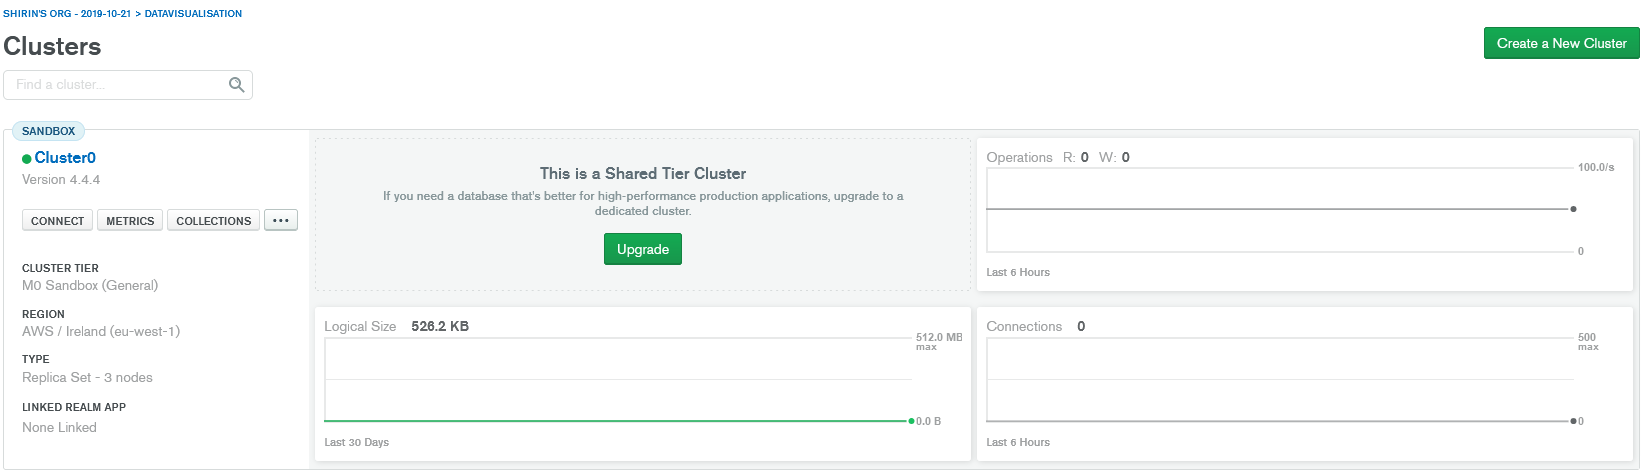
\includegraphics[scale=0.5]{img/clusterDB.PNG}
\end{center}

\section{Languages Used}
\subsection{JavaScript}
JavaScript is high-level, often just-in-time compiled, and multi-paradigm. It has curly-bracket syntax, dynamic typing, prototype-based object-orientation, and first-class functions.
Alongside HTML and CSS, JavaScript is one of the core technologies of the World Wide Web. Over 97\% of websites use it client-side for web page behavior, often incorporating third-party libraries. All major web browsers have a dedicated JavaScript engine to execute the code on the user's device.
As a multi-paradigm language, JavaScript supports event-driven, functional, and imperative programming styles. It has application programming interfaces (APIs) for working with text, dates, regular expressions, standard data structures, and the Document Object Model (DOM).
The ECMAScript standard does not include any input/output (I/O), such as networking, storage, or graphics facilities. In practice, the web browser or other runtime system provides JavaScript APIs for I/O.
JavaScript engines were originally used only in web browsers, but they are now core components of other software systems, most notably servers and a variety of applications.[SN 9]
\subsection{JSX}
JSX is an extension of Javascript and stands for JavaScript XML.
JSX allows us to write HTML elements in JavaScript and place them in the DOM without any createElement()  and/or appendChild() methods. JSX converts HTML tags into react elements.[SN 10]
React encourages the use of JSX for development, though a developer could use JavaScript if preferred.
The team used JFX for the project.

\subsection{Python}
Python is an interpreted, high-level and general-purpose programming language. Python's design philosophy emphasizes code readability with its notable use of significant indentation. Its language constructs and object-oriented approach aim to help programmers write clear, logical code for small and large-scale projects.
Python is dynamically-typed and garbage-collected. It supports multiple programming paradigms, including structured (particularly, procedural), object-oriented and functional programming.[SN 11]
Flask is written in python, the api backend of the project is written on python code. All api routes use Flask Blueprint().
Flask Blueprints encapsulate functionality, such as views, templates, and other resources. To get a taste for how a Flask Blueprint would work, you can refactor the previous application by moving the index view into a Flask Blueprint. To do so, you have to create a Flask Blueprint that contains the index view and then use it in the application.[SN 12]

\section{Development Environment}
\subsection{Visual Studio Code}
Visual Studio Code is a lightweight but powerful source code editor which runs on your desktop and is available for Windows, macOS and Linux. It comes with built-in support for JavaScript, TypeScript and Node.js and has a rich ecosystem of extensions for other languages (such as C++, C\#, Java, Python, PHP, Go) and runtimes (such as .NET and Unity).[SN 12] \url{https://code.visualstudio.com/docs}
According to Visual Studio Code,"Visual Studio Code combines the simplicity of a source code editor with powerful developer tooling, like IntelliSense code completion and debugging.
First and foremost, it is an editor that gets out of your way. The delightfully frictionless edit-build-debug cycle means less time fiddling with your environment, and more time executing on your ideas."[SN 13]
The team agrees, VS code is extremely easy to use, is much faster than other IDE's, the inbuilt support for JS and Node.js is something we considered, it also allowed us to develop the backend which was written in python, it allowed seamless integration between the different coding languages. **** need to finesse this section *******


\section{FireBase}
Firebase is a Backend-as-a-Service that was founded in 2011 that provided developers an API that enables integration of online chat functionality into their websites. 

In 2014, Google acquired Firebase and has since built it into a full fledged mobile and web development platform with over 19 different products and services with more than 1.5 million developers worldwide.

Firebase uses what is known as a NoSQL database for storing data in a Realtime Database. As the name suggest this means that data is not stored in the tables and rows found in relational database management systems (RDBMS) such as Oracle Database or Microsoft SQL Server. Nor is the data accessed using Structured Query Language (SQL) statements. Instead, the data is stored in the form of a JSON object. 

JSON is an acronym for JavaScript Object Notation and it defines a syntax used to transmit data in a format that is both lightweight and easy for both humans and software to read, write and understand.

JSON objects typically consist of a key/value pair, where the key uniquely identifies the object within the database and the value represents the data that is being stored. Multiple JSON objects are structured in the form of a JSON tree.

The Firebase SDK supports programming in C++, Java, JavaScript, JavaScript/Node.js, Objective-C, and Swift. Angular, Backbone, Ember and React are supported through bindings to the database.

\begin{figure}
    \centering
    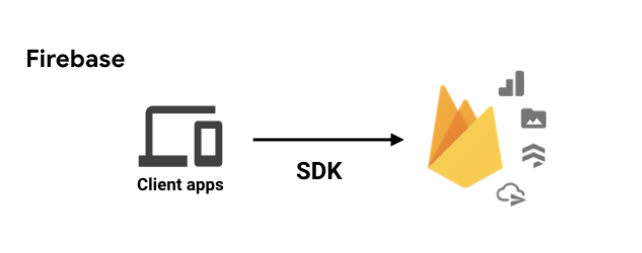
\includegraphics[scale=0.7]{img/firebase2.PNG}
    \caption{hosted in the cloud}
    \label{fig:my_label4}
\end{figure}


\subsection{User Authentication}


\begin{figure}
    \centering
    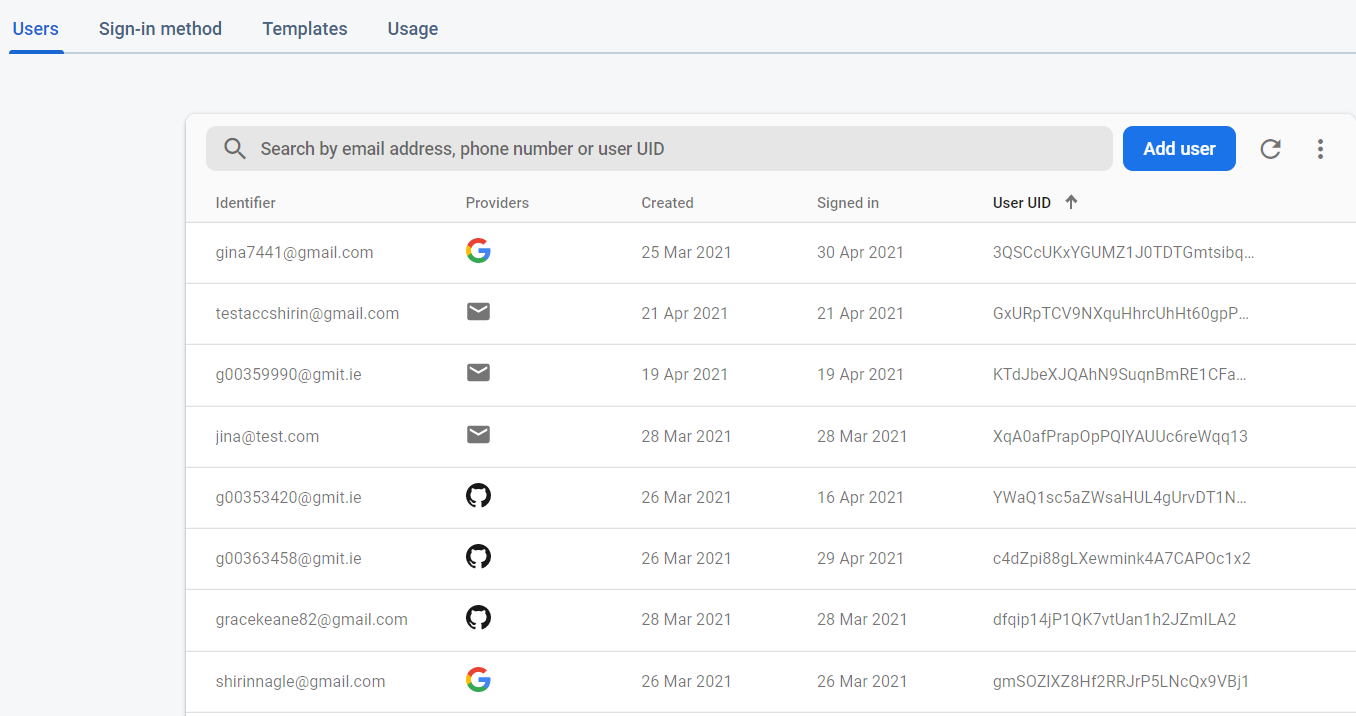
\includegraphics[scale=0.5]{img/auth.PNG}
    \caption{User data to the Database}
    \label{fig:my_label4}
\end{figure}

Firebase Authentication provides backend services, easy-to-use SDKs, and ready-made UI libraries to authenticate users to our app.

It supports authentication using email and password accounts, phone auth, Google, Facebook, Twitter, and GitHub login, and more. The Firebase Authentication (SDK) can be used to manually integrate one or more sign-in methods into an app.

To sign a user into our app, we first get authentication credentials from the user. 
These credentials can be the user's email address and password, or an OAuth token from a federated identity provider. Then, we pass these credentials to the Firebase Authentication SDK. 

Our backend services will then verify those credentials and return a response to the client.
After a successful sign in, it will allow the navigation of sensitive routes.
Authenticated user will access routes that previously locked.

\begin{figure}
    \centering
    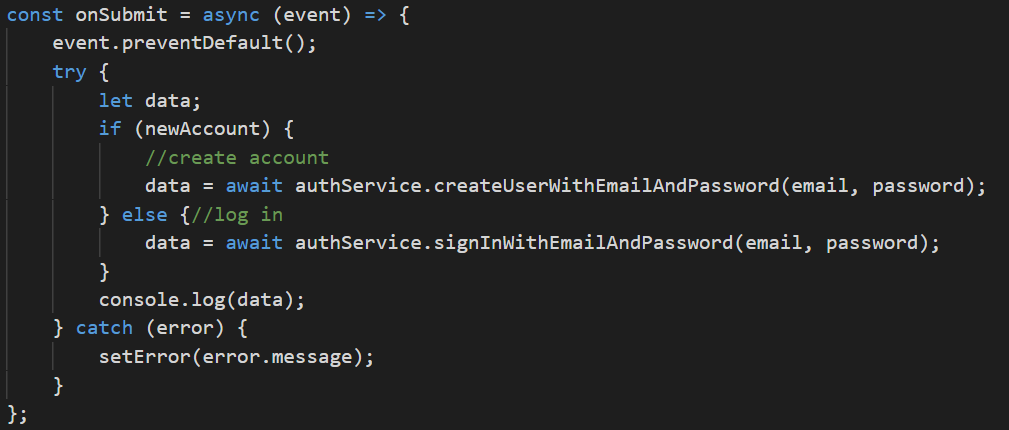
\includegraphics[scale=0.55]{img/login.PNG}
    \caption{user login and identity}
    \label{fig:my_label4}
\end{figure}


\subsection{Realtime database}

\begin{figure}
    \centering
    \includegraphics[scale=0.4]{img/Firebasedb.PNG}
    \caption{Storing and managing our data}
    \label{fig:my_label4}
\end{figure}


The Firebase Realtime Database is a cloud-hosted NoSQL database.
Data is synced across all clients in real-time and remains available even when an app goes offline.
Whenever you update data in the real-time database, it stores the data in the cloud and simultaneously notifies all interested devices in milliseconds. The real-time database is also optimized for offline use.
Whenever a user loses thier connection, the database STK uses a local cache on the device to serve and store changes. This means that when the user comes back online, their local data is automatically synchronized. To keep our data secure, we used database security rules.
The security rules are securely stored with the real-time database on our server.

I wanted to use Mers and Sars data to display D3 graphs for our group project.
I couldn’t find an API that gave me the data I wanted, but I was able to find all the data I needed in CSV format. 
I parsed all that CSV data into JSON and used Firebases’ Command-line interface to upload all the data into the server.


\section{Cloud Firestore}
Cloud Firestore is Firebase's fully managed cloud-native NoSQL document database that is fast and serverless. It's a new and improved version of the Real-Time Database, and its capabilities include real-time updates, offline synchronization, scalability, and multi-region deployment. Unlike a SQL database, there are no tables or rows. Instead, you store data in documents, which are organized into collections. Each document contains a set of key-value pairs.
Cloud Firestore is optimized for storing large collections of small documents.
All documents must be stored in collections. Documents can contain subcollections and nested objects, both of which can include primitive fields like strings or complex objects like lists.


We used Cloud Firestore for our Message Board.

User identity is an important security concept. Different users have different data, and sometimes they have different capabilities.

For example each message is associated with the user that created it. Users may also be able to delete their own messages, but not messages posted by other users.

The SDK handles all the state management and data syncing in between the client and server. I set up a collection of messages and then for each of these messages create a sub collection of messages.

If we look at the actual database we can see that each message has an owner and then each individual message is an object.

\begin{figure}
    \centering
    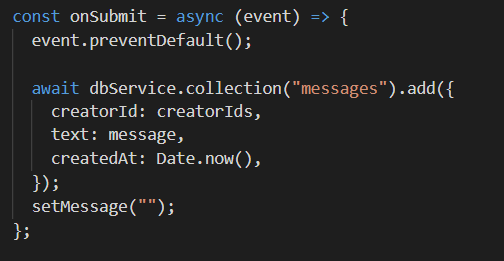
\includegraphics[scale=0.75]{img/message.PNG}
    \caption{How we manage messages}
    \label{fig:my_label4}
\end{figure}

\begin{figure}
    \centering
    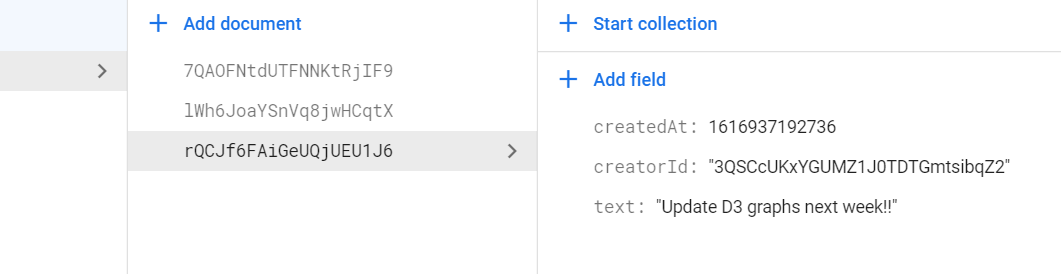
\includegraphics[scale=0.6]{img/FirestoreMessage.PNG}
    \caption{Storing and managing messages}
    \label{fig:my_label4}
\end{figure}

It contains the user ID, a created timestamp and the message content.
When a user is logged in and they created a new message it will create this document with their user ID as the owner ID.

\section{D3}


\begin{figure}
    \centering
    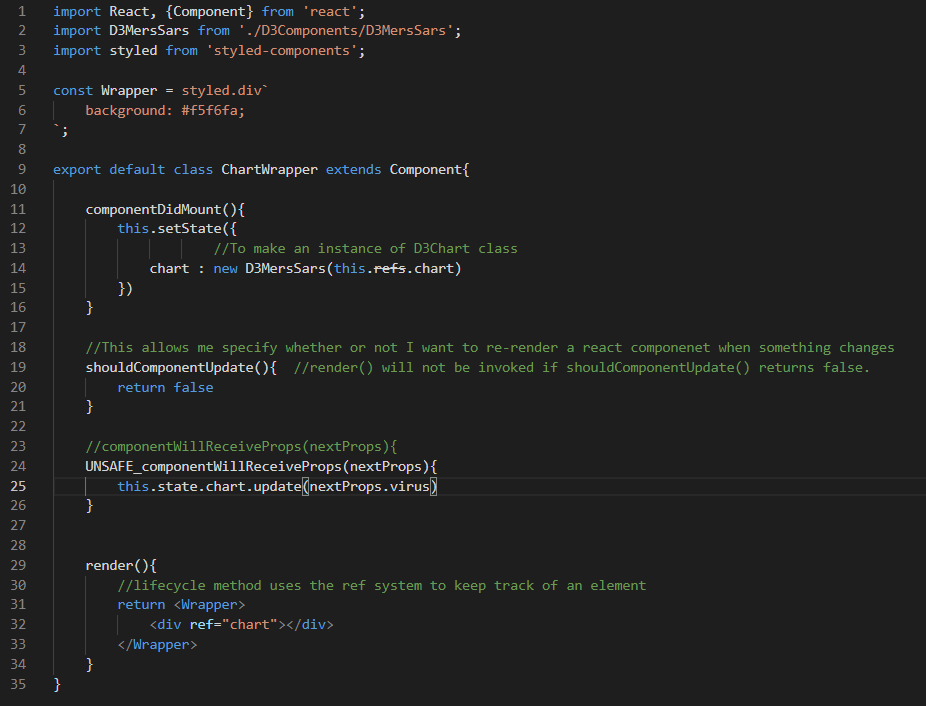
\includegraphics[scale=0.6]{img/D3Ref.PNG}
    \caption{How to access D3}
    \label{fig:my_label4}
\end{figure}

D3.js (Data-Driven-Documents) is an open-source JavaScript library that lets you create dynamic data visualizations in web browsers using SVC, HTML 5, and CSS.
Most data visualization tools require Python, D3.js visualizations are created entirely using JavaScript.

While most charting libraries (such as Chart.js and Highcharts) provide ready made charts D3 consists of a large set of building blocks from which custom charts or maps can be constructed.

D3’s approach is much lower level than other charting libraries. Creating a bar chart with Chart.js is just a few lines of code.

Creating the same chart with D3 you need to:

\begin{itemize}

\item \textbf{create SVG rect elements and join them to the data}
\item \textbf{position the rect elements}
\item \textbf{size the rect elements according to the data}
\item \textbf{add axes}

\end{itemize}


In order to \textbf{use DOM in React directly}, I used refs.

It takes two simple steps:

\begin{itemize}

\item \textbf{creating a ref in constructor()}
\item \textbf{connecting [div] to the ref}

\end{itemize}

Our ChartWrapper.js will look like this :


\chapter{System Design}
\begin{center}
      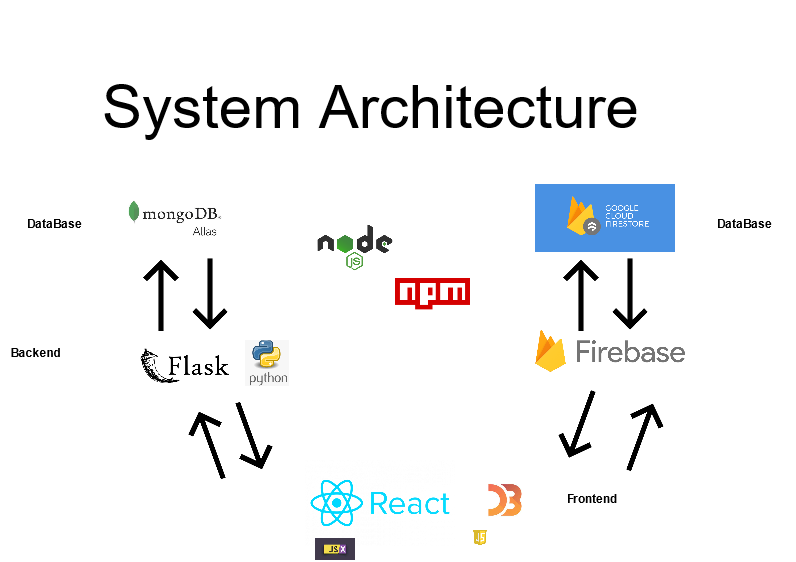
\includegraphics[scale=0.5]{img/basic architecture.png}
\end{center}

\section{Architecture Overview}
The architecture of the project is a three tiered architecture, consisting of a front-end, a back-end and a data tier.
Three-tier architecture is a well-established software application architecture that organizes applications into three logical and physical computing tiers: the presentation tier, or user interface; the application tier, where data is processed; and the data tier, where the data associated with the application is stored and managed.
The chief benefit of three-tier architecture is that because each tier runs on its own infrastructure, each tier can be developed simultaneously by a separate development team, and can be updated or scaled as needed without impacting the other tiers.[SN 0]


The front end was worked on initially, once the front-end was functioning a decision was made about the architecture of the project. Flask was decided on as the back-end, which would interact with the database tier and the front-end.
Once the architecture was finalised, we wrote our own api calls to the database.


The front end was worked on initially, once the front-end was functioning a decision was made about the architecture of the project. Flask was decided on as the back-end, which would interact with the database tier and the front-end.
Once the architecture was finalised, we wrote our own api calls to the database.

While researching mongoDB and Flask working together, we found articles on the web that described the stack were developing it was called FReMP. Unlike MEAN or MERN this acronym seems to be new and does not have as much documentation. Our architecture also includes a login facility using Firestore and some of the static data for the components rendering D3 data is stored in Firebase.

FReMP stack is a very powerful and highly scalable stack which reduces complexity of back-end code, deals with the database requests very quickly and brings a user friendly interface for front-end users.

We had decided on Flask because React does not tie a developer to use a particular back-end, and we wanted to learn more about Flask and python, which we had some familiarity with.



\section{Three tier architecture}
\subsection{Data Tier}
We chose a cloud based database MongoDB Atlas to manage some of the data required for the project. The project relies on daily updated apis for Covid19 data, as part of the initial project we investigated other pandemics and epidemics.Fortunately these occurred years ago, unfortunately it meant that the data was not easy to find. We found some limited data on SARs MERs and Smallpox. The smallpox data was stored in MongoDB and the SARs and MERs data was stored in Firebase.
Firebase was used for data that rendered D3 images. External api's were used for the Covid-19 data. The app allows a user to record temperature, symptoms and leave a rating or review, this information is stored in MongoDB and can be retrieved. Everytime the a temperature is entered a temperature graph dynamically changes.

\section{Logic Tier - Back end}
Using RESTful API's which follow an architecture that use predefined and stateless operations to access web resources.
The API is written with Flask, uses Pymongo, a python library specifically for interacting with a Mongo database. . Also firebase/firestore?
Requests from the app are sent by a request from the code in the front end, using JavaScript or JSX to the RESTful API, this API sends a connection request to MongoDB Atlas which is on the web. Flask retrieves the information and sends it to the be displayed at the application end.
Flask

\section{Application Tier Front end}
React was used to develop the client side of the application. React is an open source JavaScript library for rendering views. React apps are an example of single application applications(SPA), the application code, like HTML, CSS and Javascript is loaded once. The SPA only sends what the user needs, for example by clicking on a button only the information associated with that button is reloaded not the whole page. This piece by piece, client side method makes load time must faster for users and makes the amount of information a server has to send a lot less.
When a user interacts with the app JavaScript intercepts the browser events
More info about this element of the project goes here.
\begin{center}
      
\includegraphics{img/fremp.PNG}
\end{center}

\begin{itemize}
\item Flask
\item React.js
\item MongoDB Atlas
\item Python


These technologies were chosen as they give developers the ability to handle large volumes of data and, at the same time, render a nice modern interface on the client side.
\item Architecture, UML etc. An overview of the different components of the system. Diagrams etc… Screen shots etc.
\end{itemize}

\section{Heroku - Deployment}
\begin{center}
      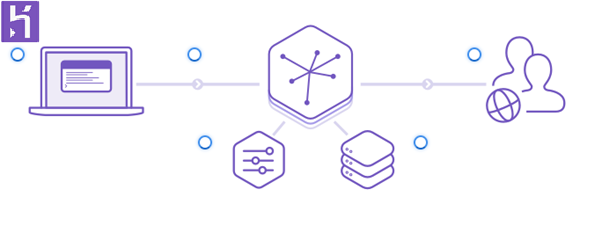
\includegraphics{img/HerokuArchitecture.png}
\end{center}
Heroku is a platform as a service based on a managed container system, with integrated data services and a powerful ecosystem, for deploying and running modern apps. [SN 14]
We deployed the project to the web using Heroku. We investigated different options for deployment, there are many companies that offer a free option or trial PaaS product, companies like Plesk, Cloudify and Heroku, as well as Open Source Paas tools.The project deployment was implemented towards the end of project development, because we had prior experience with Heroku and limited time we decided to try Heroku first. If we felt that Heroku was not suitable we would try another platform like Plesk or an open source option like Dokku, but Heroku worked well and with the time frame left we decided there was no need to investigate another option. Heroku's free option was sufficient for our app deployment.
\begin{center}
      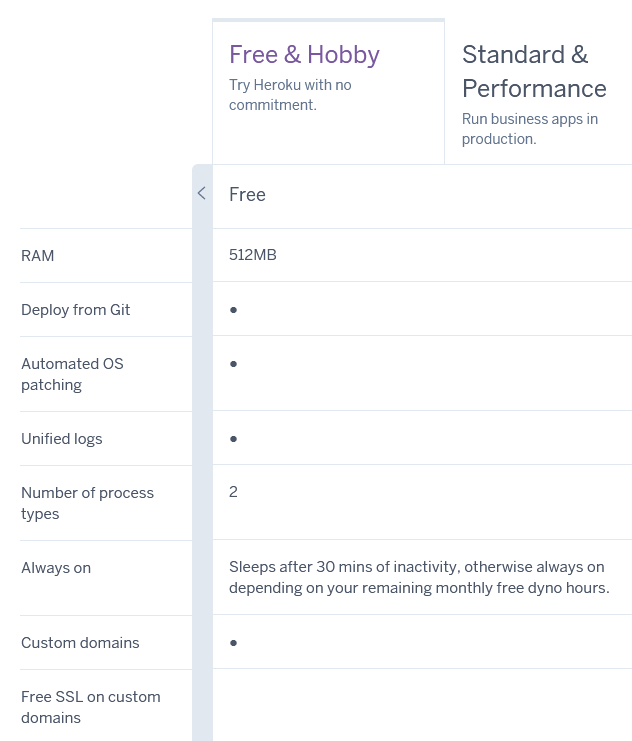
\includegraphics[scale=0.6]{img/HerokuStats.PNG}
\end{center}

\begin{table}[ht]
  \centering
  \begin{tabular}{x{2cm}p{3cm}}
    \toprule \\
    Column 1 & Column 2 \\
    \midrule \\
    Rows 2.1 & Row 2.2 \\
    \bottomrule
  \end{tabular}
  \caption{A table.}
  \label{table:mytable}
\end{table}

\chapter{System Evaluation}

\section{Chapter Overview}
In the System Evaluation chapter we will touch on the overall design of the system.
We will evaluate whether or not the objectives were met in the completion of the web application.
The testing that went into the project will also be documented.
We will also be reviewing any limitations and areas of improvement within this project.

\section{Project Objectives}
Initially the goal of this project was to develop a data visualization website that analyses various viruses such as Covid-19, Sars, Mers and Smallpox using different technologies.

\section{Testing}
This section will discuss how the application was tested.
The entire system was fully tested to ensure that there were no faults in our web application.
We felt that it was essential to fully test our web application in the development as well as in the completion of the project.
Some of the testing that we conducted included Unit Testing and System Testing.


\subsection{Unit Testing}
Unit Testing is a type of software testing where individual units or components of a software are tested. 
The purpose is to validate that each unit of the software code performs as expected.

A unit may be an individual function, method, procedure, module, or object.
The reason that it is done this way is to verify that each unit of our application is working correctly.


\subsubsection{jest}
Jest is a JavaScript unit testing framework, used by Facebook to test services and React applications.
Jest also provides Snapshot testing, the ability to create a rendered ‘snapshot’ of a component and compare it to a previously saved ‘snapshot’. The test will fail if the two do not match.

Jest was used to test both Firebase and Firestore functions.
Every time I used Firebase, I ran into the problem of how to test Firebase's database and authentication. Since I am using Jest as my default testing environment, I figured everything I needed already comes with Jest.

\begin{figure}
    \centering
    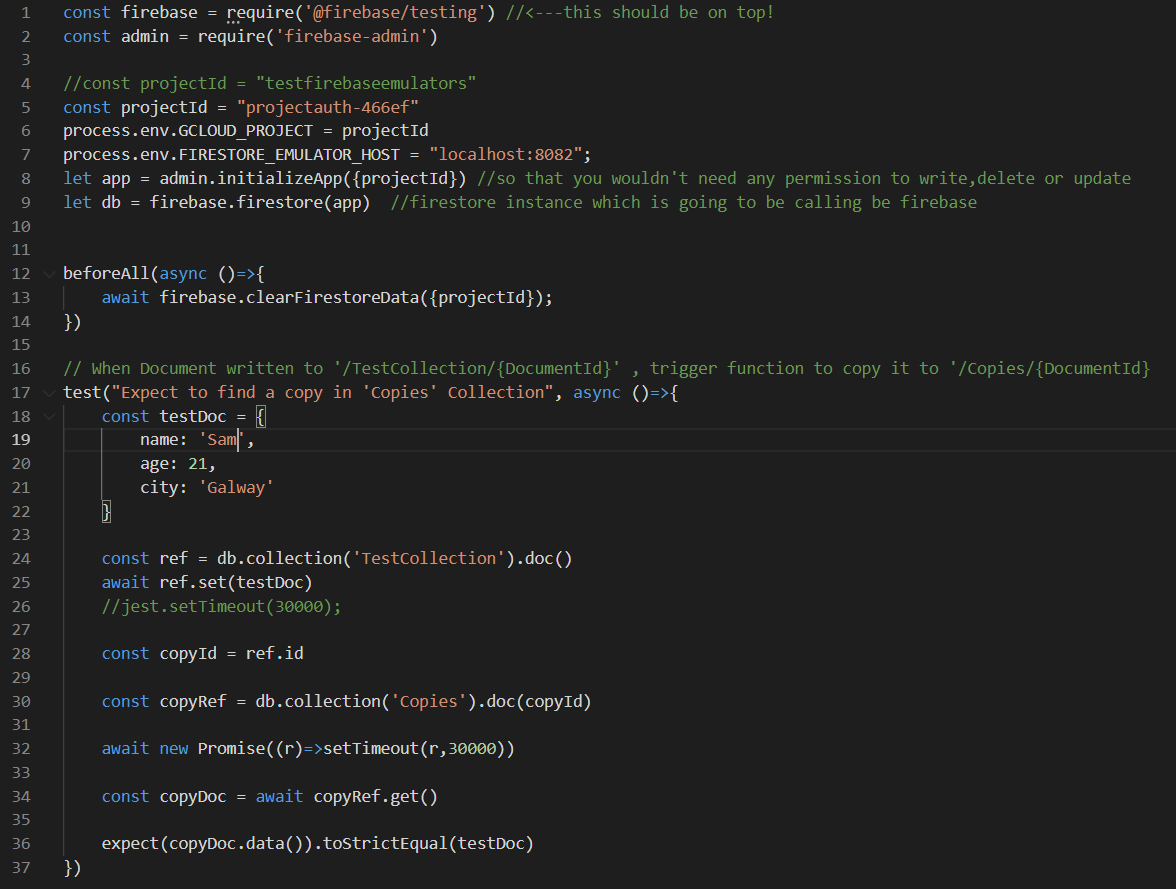
\includegraphics[scale=0.5]{img/jest.PNG}
    \caption{Testing with Jest}
    \label{fig:my_label4}
\end{figure}

\subsubsection{Firebase Emulators}
The Firebase Local Emulator Suite consists of individual service emulators built to accurately mimic the behavior of Firebase services. This means we can connect our app directly to these emulators to perform integration testing or QA without touching production data.

The Firebase Emulators make it easier to fully validate the app's behavior and verify our Firebase Security Rules configurations.
We used the Firebase Emulators to run and automate unit tests in a local environment. 

\begin{figure}
    \centering
    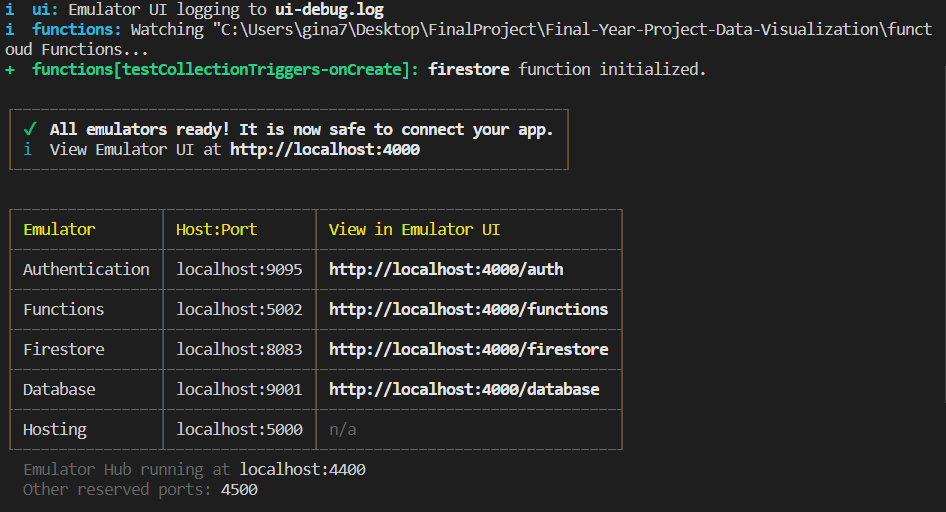
\includegraphics[scale=0.6]{img/FirebaseEmulator.PNG}
    \caption{Testing with Firebase Emulator}
    \label{fig:my_label4}
\end{figure}

\subsubsection{PyTest}
PyTest is a testing framework that allows users to write test codes using Python programming language. It helps you to write simple and scalable test cases for databases, APIs, or UI. PyTest is mainly used for writing tests for APIs. It helps to write tests from simple unit tests to complex functional tests.

\subsection{System Testing}

\subsubsection{Selenium}
Selenium is a portable framework for testing web applications. This allows the user to create tests which will monitor the users actions performed and log them so that these tests can be run and re-run with the click of a button.

\section{Limitations and areas of Improvement in this project}

\subsection{Limitations}
It is essential for us to have the application up and running on the cloud. As of now the biggest limitation we are facing is not having our flask back-end working properly with Heroku. 
Currently our application works locally. Some of the functionalities that are required flask aren't displaying with Heroku, such as our rating and checking temperature functionalities.


\subsection{Improvements}
Improvements that can be made to the current system could include adding more features. Initially, we had an idea of having an online symptom checker by using a chatbot powered by artificial intelligence. The user could diagnose symptoms for signs of Covid-19.


\chapter{Conclusion}
About three pages.

\begin{itemize}
\item Briefly summarise your context and objectives (a few lines).
\item Highlight your findings from the evaluation section / chapter and any opportunities identified.
\end{itemize}

\chapter{References Technology Review}
[SN 0] Three tier architecture; \url{https://www.ibm.com/cloud/learn/three-tier-architecture}
[SN 1] Git; \url{https://git-scm.com/}
[SN 2] GitHub; \url{https://guides.github.com/activities/hello-world/}
[SN 3] Flask; \url{https://en.wikipedia.org/wiki/Flask_(web_framework)}
[SN 4] Virtual environments; \url{https://flask.palletsprojects.com/en/1.1.x/installation/}
[SN 5] React;  \url{https://reactjs.org/}
[SN 6] Table information; \url{https://insights.stackoverflow.com/survey/2020#most-loved-dreaded-and-wanted}
[SN 7] MongoDB; \url{https://www.mongodb.com/nosql-explained}
[SN 8]
[SN 9] JavaScript; \url{https://en.wikipedia.org/wiki/JavaScript}
[SN 10] JSX; \url{https://www.w3schools.com/react/react_jsx.asp}.
[SN 11] Python; \url{https://en.wikipedia.org/wiki/Python_(programming_language)}
[SN 12] Blueprint; \url{https://realpython.com/flask-blueprint/}
[SN 13] Visual Studio Code; \url{https://code.visualstudio.com/docs/editor/whyvscode}
[SN 14] Heroku; \url{https://www.heroku.com/platform}
[SN 15] Firebase Authentication; \url{https://firebase.google.com/products/auth}
[SN 17] Firebase Database; \url{https://firebase.google.com/products/realtime-database}
[SN 18] Firestore; \url{https://firebase.google.com/products/firestore}
[SN 19] D3; \url{https://www.educative.io/blog/d3js-tutorial}
[SN 20] Unit Testing; \url{https://en.wikipedia.org/wiki/Unit_testing}
[SN 21] Firebase Emulators; \url{https://firebase.google.com/docs/rules/unit-tests}
[SN 22] Jest; \url{https://en.wikipedia.org/wiki/Jest_(JavaScript_framework)}
[SN 23] PyTest; \url{https://thinkpalm.com/blogs/pytest-a-python-solution-for-test-automation/}
[SN 24] Selenium; \url{https://en.wikipedia.org/wiki/Selenium_(software)}
[SN 25] firebase; \url{https://codeburst.io/firebase-spend-more-time-developing-the-features-that-actually-matter-814f57a499af}
